% \documentclass[Japanese]{dicomopapers}
\documentclass[Japanese,noauthor]{dicomopapers}

\usepackage[dvips]{graphicx}
\usepackage{latexsym}

\def\Underline{\setbox0\hbox\bgroup\let\\\endUnderline}
\def\endUnderline{\vphantom{y}\egroup\smash{\underline{\box0}}\\}
\def\|{\verb|}
\def\newblock{\hskip .11em plus .33em minus .07em}

\begin{document}

% 和文表題
\title{ディスプレイを用いて光電脈波センサに\\任意の脈波を計測させる手法の提案}
% 英文表題
% \etitle{DICOMO2021 Paper Format (optional)}

% 所属ラベルの定義
\affiliate{Rits}{立命館大学大学院情報理工学研究科}
\affiliate{JST}{科学技術振興機構さきがけ}

\author{藤井 敦寛}{ATSUHIRO FUJII}{Rits}[atsuhiro.fujii@iis.ise.ritsumei.ac.jp]
\author{村尾 和哉}{KAZUYA MURAO}{Rits,JST}[murao@cs.ritsumei.ac.jp]

\begin{abstract}
  ウェアラブルデバイスに関する研究は活発に行われており,様々な形状,装着部位のデバイスが提案されている.ウェアラブルデバイスは自身の生体情報を記録するために利用される場合が多く,取得されたデータから身体異常を検知する手法も提案されている.脈波データは生体情報として記録される情報の一つである.脈波センサは機構の特性上,データの取得に血流を必要とする.義手やロボットアームなど人工的な身体にスマートウォッチを装着する場合,血流が存在しないため正しいデータが取得できない.そこで,ディスプレイを用いて脈波センサに脈波データを計測させる手法を検討する.本手法が実現すれば,身体と義手の接合部などで計測された脈波を入力することで,その値をスマートウォッチに読み取らせることが可能となる.本研究では,アプローチの実現可能性を調査するために,ディスプレイの色調を変化させることで,脈波センサの取得値を意図的に操作することが可能であるか調査した.予備実験として,ディスプレイの色調を変化させながらディスプレイ上に設置した脈波センサからデータを取得した.その結果,ピークの存在するデータが取得できた.したがって,脈波センサに任意の脈波データを計測させるためにディスプレイを用いるアプローチは有効であると考えられる.
\end{abstract}

% 表題などの出力
\maketitle

% 本文はここから始まる
\section{はじめに}
\label{introduction}
健康管理への意識の高まりから,自身の生体情報を記録するウェアラブルデバイスが広く普及している.記録する生体情報は活動量や呼吸数,体温などさまざまな情報があり,心拍数もそのひとつである.心拍数を取得するために用いられる脈波センサは,緑色のLEDを皮膚に照射して,血管を通して反射した光の変化から脈波を計測する光電式容積脈波記録法(PPG)と呼ばれる方式のものが一般的であり,市販のスマートウォッチに導入されている.スマートウォッチのセンサから取得できる心拍データを用いて疲労度を検出する手法を今井ら\cite{fatigue_detection}が提案しているなど,脈波センサから得られるデータを使用した研究は盛んである.

しかしながら,義手やロボットアームなど人工的な身体には血流が存在しないためスマートウォッチを生身の身体と同様に手首に装着して生体情報を計測することはできない.通話やメッセージ,時計などのスマートウォッチの機能や加速度センサやGPSなどのセンサは人工的な身体でも利用できるが,生体情報の計測はできない.このように,人工的な身体において生身の身体で利用できていたインタフェース,デザイン,プロトコルが利用できない問題がある.この問題を解決するには,現状では追加のセンサを計測可能な身体部位に装着して,何からの通信手段を用いてセンサデータを収集する必要がある.しかし,仮に収集したとしても,スマートウォッチが提供するアプリにデータを与えてサービスを利用することはハードルが高いため,スマートウォッチに搭載されているセンサに計測させたい.しかし,計測可能部位にスマートウォッチを装着すると,本来のスマートウォッチとしての機能(時計やディスプレイ表示,タッチ操作)が利用できなくなるため,スマートウォッチ本来の使用形態である手首に装着して脈拍などの生体情報を計測できるようにすることが望ましい.
\par

本研究では,ディスプレイを用いて脈波センサに脈波データを計測させる手法を検討する.ディスプレイの表示を変化させることで任意の脈波データを脈波センサに読み取らせることができれば,義手やロボットアームなどの人工的な身体にスマートウォッチを装着する場合でも,身体と義手の接合部などで計測された脈波を入力することで,その値をスマートウォッチに読み取らせることができ,スマートウォッチが提供する機能を生身の身体と同様に利用できる.また,人工的な身体にディスプレイを搭載するのみでスマートウォッチには手を加えないため,市販のスマートウォッチをそのまま利用できる.このほか,遠隔地のロボットアバタに適用すれば,操作者の生体情報をアバタの身体でも計測できるようになる.本稿では,ディスプレイによる脈波生成の予備段階として,あらかじめ収集された実際の脈波データを参考にして,ディスプレイの色調を変化させることで,任意の心拍数を計測させる手法を提案する.ディスプレイを用いて脈波センサに脈波データを計測させることができるかを確認し,提案手法の有効性を明らかにする.
\par

% 以降,\ref{related}節で関連研究を紹介する.\ref{preliminary}節で提案手法の予備実験と結果の考察を行い,\ref{future_work}節で今後の計画を述べ,最後に\ref{conclude}節で本研究をまとめる.


\section{関連研究}
\label{related}
本節ではウェアラブルデバイスのセンシング,脈波データの利用に関する研究を紹介する.

\subsection{ウェアラブルデバイスのセンシング}
% ウェアラブルデバイスが普及している
Hamら\cite{smart_wristband}はスマートグラス用の入力デバイスとして,リストバンド型のデバイスを提案している.このデバイスはタッチパネルと慣性計測ユニットを搭載しており,タッチや手首をひねるなどのモーションで操作ができる.手首にデバイスを装着することで使用できるため,ユーザは動きを制限されず,自由度が高い.また,ポインティングにはタッチパネルを使用することで,入力の安定性を向上させた.
Hernandezら\cite{bioglass}は頭部装着型のウェアラブルデバイスである,Google Glassに内蔵された加速度センサ,ジャイロセンサ,カメラから脈拍数と呼吸数を認識する手法を提案している.
Nishajithら\cite{smart_cap}は,視覚障害者の状況認識を支援するウェアラブルデバイスとして,スマートキャップの設計と実装を行った.デバイスはRaspberry Pi 3,Raspberry Pi NoIR Camera V2,イヤホン,電源から構成される.Raspberry Pi NoIR(No Infrared) Camera V2とはRaspberry Piの赤外線カメラモジュールである.この赤外線カメラで得られる画像から検出された対象物について,イヤホンを通して音声で説明する.
これらはいずれも身体部位に装着するウェアラブルデバイスに関する研究であり,様々な形状のデバイスを用いた研究が行われている.
\par
% 原文(ヘルメット)
% Hamら\cite{smart_wristband}はスマートグラス用の入力デバイスとして,リストバンド型のデバイスを提案している.このデバイスはタッチパネルと慣性計測ユニットを搭載しており,タッチや手首をひねるなどのモーションで操作ができる.手首にデバイスを装着することで使用できるため,ユーザは動きを制限されず,自由度が高い.また,ポインティングにはタッチパネルを使用することで,入力の安定性を向上させた.
% Hernandezら\cite{bioglass}は頭部装着型のウェアラブルデバイスである,Google Glassに内蔵された加速度センサ,ジャイロセンサ,カメラから脈拍数と呼吸数を認識する手法を提案している.
% Nishajithら\cite{smart_cap}は,視覚障害者の状況認識を支援するウェアラブルデバイスとして,スマートキャップの設計と実装を行った.デバイスはRaspberry Pi 3,Raspberry Pi NoIR Camera V2,イヤホン,電源から構成される.Raspberry Pi NoIR(No Infrared) Camera V2とはRaspberry Piの赤外線カメラモジュールである.この赤外線カメラで得られる画像から検出された対象物について,イヤホンを通して音声で説明する.
% これらはいずれも身体部位に装着するウェアラブルデバイスに関する研究であり,さまざまな形状のデバイスを用いた研究が行われている.特に,頭部装着型のウェアラブルデバイスとしては帽子型や眼鏡型などが存在するが,ヘルメットを用いた研究は筆者らの知る限り存在しない.

さらに,デバイスの装着部位も多岐にわたる.
Vahdatpourら\cite{localization_vahdatpour}は25人の被験者に頭部,胸部,両上腕,両前腕,腰部,両大腿部,両脛部の計10箇所に加速度センサを装着してもらい,日常行動下の加速度データを収集した.収集したデータからSVM(Support Vector Machine)を用いて,平均89\%の精度で装着部位を推定した.
Timoら\cite{localization_timo}は15人の被験者の頭部,胸部,左上腕,左手首,腰部,ズボンの左ポケット,左足首の計7箇所に加速度センサを装着し,様々な身体活動における加速度データを収集した.収集したデータからRandom Forestを用いて装着部位を推定し,平均89\%の精度を達成した.
Kunzeら\cite{localization_kunze}は6人の被験者の右手首,右目付近の側頭部,ズボンの左ポケット,左胸のポケットの計4箇所に加速度センサを装着し,歩行動作におけるデータを収集した.収集したデータからC4.5分類木を用いて装着部位を推定した.
また,筆者ら\cite{localization_yoshida}はウェアラブルデバイスで取得可能な生体情報である心電と脈波を利用し,特定の行動を装着者に行わせることなくウェアラブルデバイスの装着部位を推定する手法を提案している.
\par
% 原文(DICOMO2020:吉田さん)
% ウェアラブルデバイスの装着位置を推定する研究として,Vahdatpourら\cite{Vahdatpour}は25人の被験者の頭部,胸部,両上腕,両前腕,腰部,両大腿部,両脛部の計10箇所に加速度センサを装着してもらい,歩行行動などの日常行動下で加速度データを収集した.収集したデータからSVM(Support Vector Machine)を用いて,平均84\%の精度で装着部位を推定している.
% Timoら\cite{Timo}は15人の被験者の頭部,胸部,左上腕,左手首,腰部,服の前ポケット,左足首の計7箇所に加速度センサを装着してもらい,歩行や走るなどの行動の加速度データを収集した.収集したデータからRandom Forestを用いて装着部位を推定し,平均89\%の精度を得ている.
% Kunzeら\cite{Kunze}は6人の被験者に右手首,右目の横,ズボンの左ポケット,左胸のポケットに加速度センサを装着してもらい,歩行動作のデータを収集した.収集したデータからC4.5分類木を用いて装着部位を推定し,平均94\%の精度を得ている.

このように,ウェアラブルデバイスは様々な形状のものが提案されており,装着部位も広範囲であることから,活発な研究が行われている.


\subsection{脈波データの利用}
ウェアラブルデバイスは生体情報を取得するために用いられる.Spinsanteら\cite{accuracy_in_low_intensity}は低強度の身体活動時にスマートウォッチから取得される心拍数に注目し,その精度を計測している.Hanら\cite{arrhythmia_detection}はスマートウォッチから取得された脈波データから心房期外収縮(PAC)および,心室性期外収縮(PVC)を検出する手法を提案している.
これらはウェアラブルデバイスから取得された脈波データを用いた研究である.人工的な身体ではウェアラブルデバイスを装着しても生体情報を収集できないため,これらの応用を利用できない.これに対して筆者らは人工的な身体であったとしてもウェアラブルデバイスにセンサデータを計測させることで,生身の身体と同様にこれらの応用を利用できるようにするものである.

% \subsection{脈波センサの制御}
% % 脈波データの制御において,人体を使わないという新規性
% % 澤野さんのも入れたいが未発表?
% 筆者ら\cite{akimoto}は身体を圧迫することで血流変化を生み出し,脈波センサへの入力を改変することでコマンド入力を可能とする入力インタフェースを提案している.
% \par

% 本研究では脈波センサの入力において身体を使用しない.そのため,義手やロボットアームへの使用も可能である.





\section{予備実験}
\label{preliminary}
本節では,提案手法の実現可能性を調査するため行った予備実験について説明する.予備実験として,ディスプレイ上に脈波センサを貼り付けた状態で,ディスプレイの色調を変化させたときの脈波センサの取得値を観察した.


\subsection{データ収集}
事前に実際の脈波データを20代男性1名から収集した.\figref{fig:sensors}の左図に示すように,左手人差し指に光電式容積脈波記録法の脈波センサ(pulsesensor.com製)を装着した.脈波センサはArduinoUNOを介してPCに接続しており,サンプリング周波数は約90Hzで10秒間データの収集を行った.

\subsection{実験方法}
データ収集で使用したPCとは異なるPC(SurfaceLaptop)のディスプレイの色調を変化させた.\figref{fig:sensors}の右図に示すように,ディスプレイ上に脈波センサを乗せ,光が入らないように布で覆ったあと,ガムテープで固定した.事前に脈波データを収集したときと同じ条件でデータの取得を行った.ディスプレイの色調の変化にはJavaScriptを使用し,ブラウザの背景色を変化させることで制御した.事前に収集した脈波データを1サンプルずつ読み込み,その値に応じた3色で表示を繰り返す.全サンプルの処理が終了した場合,同じデータで再び処理を行う.
\par

表示する色は,次式により定義した.
\begin{equation}
  \label{eqn:low}
  value < \theta_{1} \quad (\theta_{1}=465)
\end{equation}

\begin{equation}
  \label{eqn:middle}
  \theta_{1} \leq value \leq \theta_{2} \quad (\theta_{1}=465, \theta_{2}=685)
\end{equation}

\begin{equation}
  \label{eqn:high}
  \theta_{2} < value \quad (\theta_{2}=685)
\end{equation}
式\ref{eqn:low}を満たす場合はR:150, G:19, B:20,式\ref{eqn:middle}を満たす場合はR:157, G:26, B:27,式\ref{eqn:high}を満たす場合はR:156, G:25, B:26で表現される色を表示する.また,1サンプルを読み込み,色を表示するごとに10msの遅延を挟んだ.

\begin{figure}[!t]
  \begin{center}
    \includegraphics[width=1\linewidth]{figures/sensors.eps}
  \end{center}
  \caption{脈波データの取得方法}
  \label{fig:sensors}
\end{figure}


\subsection{結果と考察}
取得された脈波データを,最初のピークから5秒間切り出した結果を\figref{fig:pulse}に示す.結果から,ピークを生成できていることが確認できる.したがって,ディスプレイを使用するアプローチは有効だといえる.しかしながら,ピークの位置や値に違いが見られる.これは,ディスプレイ制御の開始時刻とセンサ値の取得の開始時刻を同期していなかったことや,サンプルの処理ごとの遅延を10msに固定していたことが影響したと考えられる.

\begin{figure}[!t]
  \begin{center}
    \includegraphics[width=1\linewidth]{figures/pulse.eps}
  \end{center}
  \caption{脈波センサの取得値の変化}
  \label{fig:pulse}
\end{figure}


\section{今後}
\label{future_work}
予備実験の結果から,ディスプレイを用いて脈波センサに脈波を計測させることができることを確認した.今後は実環境での使用を想定して,身体部位から得られた実際の脈波データを入力することで,ディスプレイ上に設置した脈波センサに同一のデータを計測させる機構を実装する.この機構の想定を\figref{fig:future_work}に示す.実現するには,ディスプレイに表示する色を自動で決定し続ける必要がある.そのため,脈波データを入力することでディスプレイに表示する色を出力することができるような識別モデルを構築する.

\begin{figure}[!t]
  \begin{center}
    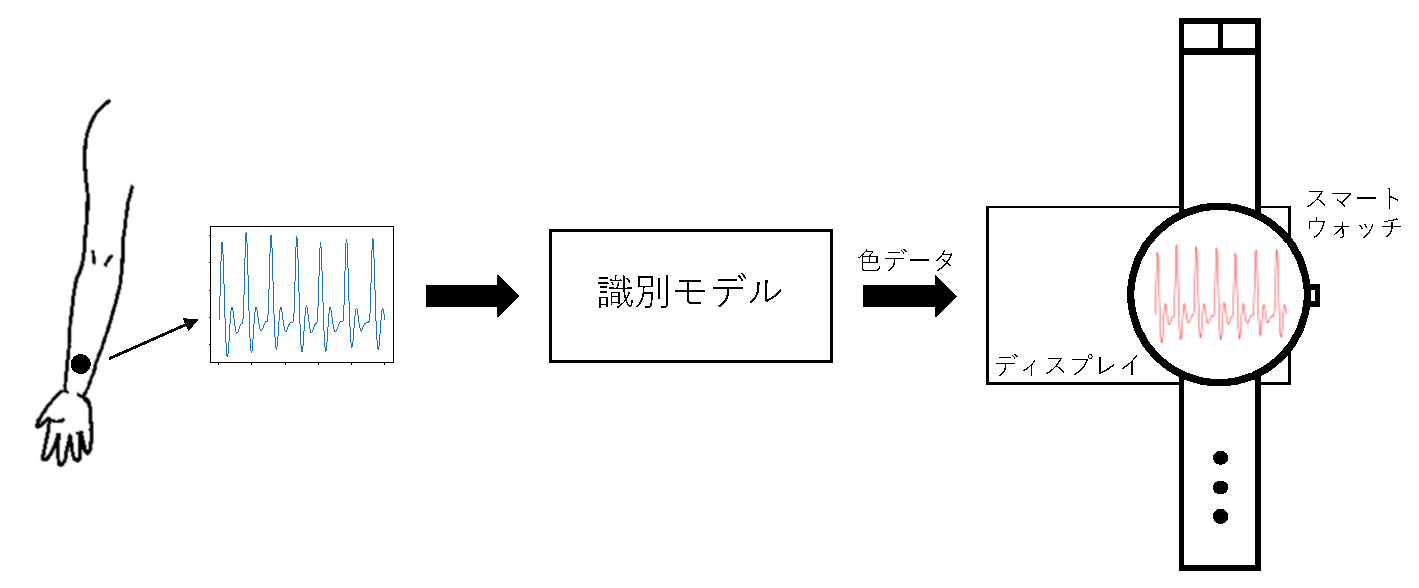
\includegraphics[width=1\linewidth]{figures/future_work.eps}
  \end{center}
  \caption{脈波センサの取得値の変化}
  \label{fig:future_work}
\end{figure}


\section{まとめ}
\label{conclude}
本研究では,ディスプレイを用いて脈波センサに脈波データを計測させる手法を実現するために,ディスプレイの色調を変化させることで,脈波センサの取得値を意図的に操作することが可能であるか調査した.予備実験として,事前に被験者1人から実際の脈波データを収集しておき,そのデータから値に応じた色調をディスプレイに繰り返し表示しながら,ディスプレイ上に設置した脈波センサからデータを取得した.予備実験の結果,ディスプレイ上の脈波センサからピークの存在するデータが取得できた.この結果から,脈波データを計測させるためにディスプレイを用いるアプローチは有効であることが確認できた.
\par

今後は,身体部位から取得された実際の脈波データを,ディスプレイを用いて再現する機構を実装する.そのためには,自動でディスプレイの色調を決定していく必要があるため,適切な識別モデルを設計していく.

\begin{acknowledgment}
  本研究は,科学技術振興機構戦略的創造研究推進事業さきがけ(JPMJPR1937)の支援を受けたものである.ここに記して謝意を表す.
\end{acknowledgment}


\bibliography{references}
\bibliographystyle{junsrt}

\end{document}
